\documentclass[12pt]{article}

\usepackage{sbc-template}
\usepackage{graphicx,url}
\usepackage[brazil]{babel}   
%\usepackage[latin1]{inputenc}  
\usepackage[utf8]{inputenc}  
% UTF-8 encoding is recommended by ShareLaTex
\usepackage{seqsplit}
\usepackage{amsmath}

\DeclareMathSymbol{\mlq}{\mathord}{operators}{``}
\DeclareMathSymbol{\mrq}{\mathord}{operators}{`'}

% Pacotes referentes às tabelas
\usepackage{longtable, multirow, array}
\usepackage{threeparttablex}


\newcolumntype{V}[1]{>{\raggedright\let\newline\\\arraybackslash\hspace{0pt}}p{#1}}
% Tipo centralizado
\newcolumntype{C}[1]{>{\raggedright\centering\let\newline\\\arraybackslash\hspace{0pt}}p{#1}}

\sloppy

\title{Codificador/decodificador convolucional usando o Algoritmo de Viterbi}

\author{Gabriel Batista Galli\inst{1}, Matheus Antonio Venancio Dall'Rosa\inst{1}, Vladimir Belinski\inst{1}}

\address{Ciência da Computação -- Universidade Federal da Fronteira Sul
  (UFFS)\\
  Caixa Postal 181 -- 89.802-112 -- Chapecó -- SC -- Brasil
  \email{\{g7.galli96, matheusdallrosa94, vlbelinski\}@gmail.com}
}

\begin{document} 

\maketitle
     
\begin{resumo} 
  O presente trabalho, apresentado ao curso de Ciência da Computação da Universidade Federal da Fronteira Sul - UFFS - Campus Chapecó - como requisito parcial para aprovação no Componente Curricular Inteligência Artificial, 2017.1, sob orientação do professor José Carlos Bins Filho, consiste na descrição da implementação de um codificador/decodificador convolucional usando o Algoritmo de Viterbi, bem como dos resultados obtidos.
\end{resumo}

\section{Introdução}

De modo geral, um código convolucional é um tipo de código corretor de erros que gera símbolos de paridade através da aplicação de uma ``janela deslizante'' (\textit{sliding window}) de uma função polinomial booleana para um fluxo de dados. A codificação convolucional é utilizada em uma variedade de sistemas, como, por exemplo, nos padrões \textit{wireless} (como o 802.11) e em comunicação via satélite \cite{MIT:2010}. Uma maneira amplamente utilizada e eficiente de se realizar a decodificação de códigos convolucionais é através da utilização do Algoritmo de Viterbi \cite{MIT:2010}.

Sabendo-se disso, no presente trabalho é apresentada a implementação de um codificador/decodificador convolucional usando o Algoritmo de Viterbi. Na Seção 2 será provida um descrição geral do processo de codificação e decodificação que serviu como base ao trabalho. Por sua vez, na Seção 3 será comentado o algoritmo criado para o atendimento da proposta, descritos os problemas encontrados durante a realização do trabalho e as soluções utilizadas. Por fim, na Seção 4 serão apresentados exemplos de codificação e decodificação alcançados pelo algoritmo desenvolvido.

\section{Descrição do processo base de codificação e decodificação}

O processo que serviu como base à implementação do codificador/decodificador convolucional desenvolvido neste trabalho é formado por quatro etapas:

\begin{enumerate}
    \item Codificação: nesta etapa é realizada a codificação da sequência de bits de entrada para um código. Para isso, faz-se uso de uma tabela de emissões e transições. O processo de codificação será melhor detalhado na subseção 2.1;
    \item Adição de ruído: nesta etapa é realizada a aplicação de ruído no código gerado a partir da etapa anterior, de forma a modificar alguns de seus bits. Esta etapa simula a ocorrência de ruídos na mensagem/ código e é necessária para a posterior verificação da capacidade do decodificador em recuperar a mensagem original mesmo caso essa apresente uma determinada quantidade de erros;
    \item Decodificação: nesta etapa é realizada a decodificação do código resultante da Etapa 2, utilizando-se para tal o Algoritmo de Viterbi. O processo de decodificação será melhor detalhado na subseção 2.2;
    \item Comparação: nesta etapa é realizada a comparação dos bits de entrada original com os bits decodificados, de forma a verificar a eficiência do algoritmo de decodificação.
\end{enumerate}

\subsection{Etapa de Codificação}

No processo de codificação têm-se que cada bit de entrada influencia a geração de três pares de bits de saída. Todavia, para cada bit de entrada são gerados apenas dois bits de saída, estes que serão considerados nas etapas de adição de ruído e decodificação. A influência mencionada ocorre devido ao fato de cada bit de entrada, além de gerar os bits de saída, também colocar o estado atual em um dos quatro possíveis estados (00, 01, 10, 11). Ademais, são gerados dois pares de bits extras no final, de modo a se utilizar toda a influência dos bits de entrada. Cabe destacar também que o estado inicial do codificador é sempre 00 e a troca de estados e emissão dos pares de bits segue o que está definido na Tabela \ref{transTable}.

\begin{table}[!h]
\centering
\caption{Tabela de emissões e transições}
\label{transTable}
\def\arraystretch{1.2}
\begin{tabular}{|c|c|c|c|c|}
\hline
\multicolumn{1}{|c|}{\multirow{2}{*}{Estado atual}} & \multicolumn{2}{c|}{Par emitido} & \multicolumn{2}{c|}{Próximo estado} \\ \cline{2-5} 
\multicolumn{1}{|c|}{} & \multicolumn{1}{c|}{Ent = 0} & \multicolumn{1}{c|}{Ent = 1} & \multicolumn{1}{c|}{Ent = 0} & \multicolumn{1}{c|}{Ent = 1} \\ \hline
00 & 00 & 11 & 00 & 10 \\ \hline
01 & 11 & 00 & 00 & 10 \\ \hline
10 & 10 & 01 & 01 & 11 \\ \hline
11 & 01 & 10 & 01 & 11 \\ \hline
\end{tabular}
\end{table}

Um exemplo de codificação pode ser verificado na Tabela \ref{encode}. Nele, têm-se como entrada a sequência de bits ``001''. A essa sequência são concatenados os bits ``00'', a fim de que sejam gerados dois pares de bits extras no final e assim seja utilizada toda a influência dos bits de entrada, como já mencionado.

\begin{table}[!ht]
\centering
\caption{Codificação da sequência de bits ``001''}
\label{encode}
\def\arraystretch{1.2}
\begin{tabular}{ccccccccccccc}
       & Entrada & & \textbf{0} & & \textbf{0} & & \textbf{1} & & 0 & & 0\\
       & & $\nearrow$ & $\downarrow$ & $\nearrow$ & $\downarrow$ & $\nearrow$ & $\downarrow$ & $\nearrow$ & $\downarrow$ & $\nearrow$ & $\downarrow$\\
Estado & 00 &  & 00 &  & 00 &  & 10 &  & 01 &  & 00\\
       & & & $\downarrow$ & & $\downarrow$ & & $\downarrow$ & & $\downarrow$ & & $\downarrow$\\
       & Saída & & 00 & & 00 & & 11 & & 10 & & 11\\
\end{tabular}
\end{table}

A codificação de ``001'' ocorre da seguinte maneira. Após a concatenação dos bits ``00'' à entrada, conforme já apresentado, toma-se 00 como estado inicial do codificador. Estando no estado atual 00 é então verificado o primeiro bit da entrada, neste caso `0', e seguida a tabela de emissões/transições apresentada na Tabela \ref{transTable} para o estado atual ``00'' e `Ent' igual ao primeiro bit de entrada (`0'), obtendo-se, assim, o par ``00'' como par de bits emitidos (saída) e o par ``00'' como próximo estado. Agora, toma-se como estado atual o par de bits obtido como próximo estado pela transição anterior, bem como considera-se o próximo bit da entrada. Com esses dados é então realizada nova consulta à Tabela \ref{transTable} a fim de se obter seus respectivos valores de par emitido (saída) e de próximo estado.  Tal procedimento é realizado até que todos os bits da entrada (inclusive os dois adicionados) sejam analisados. Por fim, toma-se a sequência de bits emitidos gerada (saída) como resultado da codificação. Pela Tabela \ref{encode} é perceptível que, para a entrada ``001'', a codificação obtida é ``00 00 11 10 11''.

\subsection{Etapa de Decodificação}

Na etapa de decodificação é utilizado o Algoritmo de Viterbi (conforme descrito abaixo), a fim de, a partir do código produzido nas etapas anteriores, descobrir-se a sequência de bits original.

Na decodificação, 00 é tomado como estado inicial. A partir dele, realizam-se transições seguindo a Tabela \ref{transTable}, bem como calcula-se para cada caminho o erro acumulado (seu cálculo será descrito em sequência). Quando há mais de um caminho para um estado, é então escolhido aquele que apresenta menor erro ou, caso ambos os caminhos apresentem o mesmo erro, escolhido um aleatoriamente. Esse procedimento é repetido até que se tenha passado por todos os pares de bit do código recebido. Por fim, é tomado o caminho com menor erro e realizado o caminho inverso, obtendo-se, assim, os estados mais prováveis e as transições que ocorreram entre eles. Para encontrar a entrada original, é feita a emissão para cada estado que a transição indica e desprezados os dois últimos valores (pois também foram adicionados dois bits à entrada original na etapa de codificação).

Um exemplo de decodificação pode ser verificado nas Tabelas \ref{decodTable1}, \ref{decodTable2}, \ref{decodTable3}, \ref{decodTable4} e \ref{decodTable5}. Nelas, é encontrada a sequência de passos para a decodificação do código ``00 00 11 10 11''. A seguir é apresentada uma descrição da decodificação de tal código.

Como já mencionado, inicia-se com o estado 00. A partir de 00 a Tabela \ref{transTable} permite que seja emitido 00 (caso a entrada seja 0) ou 11 (caso a entrada seja 1). Ademais, permite que sejam atingidos os estados 00 (caso a entrada seja 0) ou 10 (caso a entrada seja 1). Como o primeiro par recebido foi 00 e o erro é calculado pela diferença de bits do par que seria emitido pelo estado e do par recebido, somado ao erro acumulado (0 para o primeiro par recebido), temos duas opções: permanecer no estado 00 com um erro de 0, ou permanecer no estado 10 com um erro de 2. Essa situação pode ser verificada na Tabela \ref{decodTable1}.

\begin{table}[!ht]
\centering
\caption{Decodificação da mensagem 00 00 11 10 11 (primeiro par recebido)}
\label{decodTable1}
\def\arraystretch{1.2}
\begin{tabular}{cccccccc}
\multirow{2}{4.2em}{Estado Inicial} & \multirow{2}{4.2em}{Bit de Entrada} &  \multirow{2}{4.2em}{Bits Emitidos} & \multirow{2}{4.2em}{Bits Recebidos} & \multirow{2}{4.2em}{Estado Final} & \multirow{2}{4.2em}{Erro} \\&&&&&\\ \hline
 00 & 0 & 00 & 00 & 00 & 0 &\\
 00 & 1 & 11 & 00 & 10 & 2 &\\ \hline
\end{tabular}
\end{table}

O próximo par recebido foi 00. Como visto na Tabela \ref{decodTable1}, pelo primeiro par recebido podem ser alcançados como estados finais 00 e 10. Assim, para o segundo par recebido são quatro as opções de pares de estado inicial e bit de entrada: estado inicial 00 e bit de entrada 0, estado inicial 00 e bit de entrada 1, estado inicial 10 e bit de entrada 0 e estado inicial 10 e bit de entrada 1. 

As emissões, transições e erros para cada uma das opções descritas acima podem ser verificadas na Tabela \ref{decodTable2}. É importante enfatizar que nessa etapa já existe erro acumulado. Assim, as opções com estado inicial 00 tem seu erro somado ao erro da entrada com estado final 00 da Tabela \ref{decodTable1}, bem como aquelas com estado inicial 10 tem seu erro somado ao erro da entrada com estado final 10 da Tabela \ref{decodTable1}.

\begin{table}[!ht]
\centering
\caption{Decodificação da mensagem 00 00 11 10 11 (segundo par recebido)}
\label{decodTable2}
\def\arraystretch{1.2}
\begin{tabular}{cccccccc}
\multirow{2}{4.2em}{Estado Inicial} & \multirow{2}{4.2em}{Bit de Entrada} &  \multirow{2}{4.2em}{Bits Emitidos} & \multirow{2}{4.2em}{Bits Recebidos} & \multirow{2}{4.2em}{Estado Final} & \multirow{2}{4.2em}{Erro} \\&&&&&\\ \hline
 00 & 0 & 00 & 00 & 00 & 0+0=0 &\\
 00 & 1 & 11 & 00 & 10 & 0+2=2 &\\
 10 & 0 & 10 & 00 & 01 & 2+1=3 &\\
 10 & 1 & 01 & 00 & 11 & 2+1=3 &\\\hline
\end{tabular}
\end{table}

O próximo par recebido foi 11. Como visto na Tabela \ref{decodTable2}, pelo segundo par recebido podem ser alcançados como estados finais 00, 01, 10 e 11. Assim, para o terceiro par recebido são oito as opções de pares de estado inicial e bit de entrada, conforme apresentado na Tabela \ref{decodTable3}.

Cabe destacar que para o terceiro par recebido há mais de um caminho para cada estado final. Assim, para cada par com um mesmo estado final, escolhe-se a opção com menor erro ou, caso elas tenham o mesmo erro, escolhe-se uma aleatoriamente. Desta forma, é realizada uma poda nas opções a serem consideradas para o próximo par de bits recebidos, além de serem tomadas sempre as opções com menor erro e, por isso, mais próximas a uma resposta correta.

\begin{table}[!ht]
\centering
\caption{Decodificação da mensagem 00 00 11 10 11 (terceiro par recebido)}
\label{decodTable3}
\def\arraystretch{1.2}
\begin{tabular}{cccccccc}
\multirow{2}{3.6em}{Estado Inicial} & \multirow{2}{3.6em}{Bit de Entrada} &  \multirow{2}{3.6em}{Bits Emitidos} & \multirow{2}{3.6em}{Bits Recebidos} & \multirow{2}{3.6em}{Estado Final} & \multirow{2}{3.6em}{Erro} &
\multirow{2}{3.6em}{Escolhido}\\&&&&&&\\ \hline
 00 & 0 & 00 & 11 & 00 & 0+2=2 & $\longleftarrow$\\
 01 & 0 & 11 & 11 & 00 & 3+0=3 &\\
 10 & 0 & 10 & 11 & 01 & 2+1=3 & $\longleftarrow$\\
 11 & 0 & 01 & 11 & 01 & 3+1=4 &\\
 00 & 1 & 11 & 11 & 10 & 0+0=0 & $\longleftarrow$\\
 01 & 1 & 00 & 11 & 10 & 3+2=5 &\\
 10 & 1 & 01 & 11 & 11 & 2+1=3 & $\longleftarrow$\\
 11 & 1 & 10 & 11 & 11 & 3+1=4 &\\\hline
\end{tabular}
\end{table}

O próximo par recebido foi 10. Para ele, é seguido o mesmo procedimento aplicado aos pares anteriores. As emissões, transições e erros para cada uma das opções relacionadas ao quarto par recebido podem ser verificadas na Tabela \ref{decodTable4}.

\begin{table}[!ht]
\centering
\caption{Decodificação da mensagem 00 00 11 10 11 (quarto par recebido)}
\label{decodTable4}
\def\arraystretch{1.2}
\begin{tabular}{cccccccc}
\multirow{2}{3.6em}{Estado Inicial} & \multirow{2}{3.6em}{Bit de Entrada} &  \multirow{2}{3.6em}{Bits Emitidos} & \multirow{2}{3.6em}{Bits Recebidos} & \multirow{2}{3.6em}{Estado Final} & \multirow{2}{3.6em}{Erro} &
\multirow{2}{3.6em}{Escolhido}\\&&&&&&\\ \hline
 00 & 0 & 00 & 10 & 00 & 2+1=3 & $\longleftarrow$\\
 01 & 0 & 11 & 10 & 00 & 3+1=4 &\\
 10 & 0 & 10 & 10 & 01 & 0+0=0 & $\longleftarrow$\\
 11 & 0 & 01 & 10 & 01 & 3+2=5 &\\
 00 & 1 & 11 & 10 & 10 & 2+1=3 & $\longleftarrow$\\
 01 & 1 & 00 & 10 & 10 & 3+1=4 &\\
 10 & 1 & 01 & 10 & 11 & 0+2=2 & $\longleftarrow$\\
 11 & 1 & 10 & 10 & 11 & 3+0=3 &\\\hline
\end{tabular}
\end{table}

O último par recebido foi 11. Para ele, também é seguido o mesmo procedimento aplicado aos pares anteriores. As emissões, transições e erros para cada uma das opções relacionadas ao quinto par recebido podem ser verificadas na Tabela \ref{decodTable5}.

\begin{table}[!ht]
\centering
\caption{Decodificação da mensagem 00 00 11 10 11 (quinto par recebido)}
\label{decodTable5}
\def\arraystretch{1.2}
\begin{tabular}{cccccccc}
\multirow{2}{3.6em}{Estado Inicial} & \multirow{2}{3.6em}{Bit de Entrada} &  \multirow{2}{3.6em}{Bits Emitidos} & \multirow{2}{3.6em}{Bits Recebidos} & \multirow{2}{3.6em}{Estado Final} & \multirow{2}{3.6em}{Erro} &
\multirow{2}{3.6em}{Escolhido}\\&&&&&&\\ \hline
 00 & 0 & 00 & 11 & 00 & 3+2=5 &\\
 01 & 0 & 11 & 11 & 00 & 0+0=0 & $\longleftarrow$\\
 10 & 0 & 10 & 11 & 01 & 3+1=4 &\\
 11 & 0 & 01 & 11 & 01 & 2+1=3 & $\longleftarrow$\\
 00 & 1 & 11 & 11 & 10 & 3+0=3 &\\
 01 & 1 & 00 & 11 & 10 & 0+2=2 & $\longleftarrow$\\
 10 & 1 & 01 & 11 & 11 & 3+1=4 &\\
 11 & 1 & 10 & 11 & 11 & 2+1=3 & $\longleftarrow$\\\hline
\end{tabular}
\end{table}

Agora, é tomado o caminho com menor erro e feito o caminho inverso, para a obtenção dos estados mais prováveis e as transições que ocorreram entre esses. Assim, a partir da Tabela \ref{decodTable5} tem-se 00 como estado final de menor erro, este alcançado pela opção com 01 como estado inicial e 0 como bit de entrada. O mesmo é analisado nas Tabelas \ref{decodTable4}, \ref{decodTable3}, \ref{decodTable2} e \ref{decodTable1}. O caminho inverso completo, bem como a emissão para cada estado que a transição indica, pode ser conferido na Tabela \ref{return}.

\begin{table}[!ht]
\centering
\caption{Caminho inverso seguindo o menor erro}
\label{return}
\def\arraystretch{1.2}
\begin{tabular}{ccccccccccccc}
Estado & 00 & $\longleftarrow$ & 01 & $\longleftarrow$ & 10 & $\longleftarrow$ & 00 & $\longleftarrow$ & 00 & $\longleftarrow$ & 00\\
&&& $\downarrow$ && $\downarrow$ && $\downarrow$ && $\downarrow$ && $\downarrow$\\
Bit de Entrada &&& 0 & & 0 & & 1 & & 0 & & 0\\
\end{tabular}
\end{table}

Para encontrar a entrada original, além da emissão para cada estado que a transição indica, também devem ser desprezados os 2 últimos valores (pois igualmente foram adicionados dois bits à entrada original na etapa de codificação). Assim, se pela Tabela \ref{return} temos como bits de entrada a sequência ``00100'' (formada pela concatenação dos bits de entrada da direita para a esquerda -- ordem original), a entrada original decodificada é ``001''. 

\section{Descrição geral do algoritmo, dos problemas encontrados e soluções utilizadas}

A implementação do codificador/decodificador convolucional usando o Algoritmo de Viterbi descrito na seção anterior pode ser encontrada no arquivo \emph{main.cpp}.

Inicialmente, é realizada na função \emph{main()} a leitura das duas entradas necessárias ao programa: (a) a porcentagem de ruído a ser inserido no código resultante da codificação (armazenada na variável \emph{err\_percentage}); e (b) a sequência de bits de entrada (armazenada na variável \emph{bit\_sequence}). Ambos os valores devem estar contidos em um arquivo informado na compilação/execução do programa, conforme descrito no README que acompanha a implementação, sendo que este deve ser formado por duas linhas: a primeira contendo um valor de 0 a 100 indicando a porcentagem de ruído e a segunda uma sequência de bits de entrada formada por zeros e uns.

Em seguida, são realizadas chamadas à função \emph{init\_table()}, de modo a realizar a inicialização de duas estruturas de dados do tipo \emph{map}, uma que irá conter os mapeamentos referentes às emissões de pares de bit (nomeada \emph{emitted}) e outra que irá conter os mapeamentos referentes às transições de estado (nomeada \emph{next\_state}). Cabe destacar que tais estruturas seguem as emissões e transições apresentadas na Tabela \ref{transTable}.

Após isso, é feita a codificação da sequência de bits lida na entrada. Para tal, realiza-se uma chamada à função \emph{encode()}. Nela, inicialmente são concatenados os bits ``00'' ao final da sequência original de bits e definido 00 como estado inicial, tal como apresentado e justificado na subseção 2.1. Feito isso, é então realizado o processo de codificação tal qual informado na subseção 2.1, sendo o código gerado como saída retornado pela função e armazenado na variável \emph{encoded\_sequence}.

Como próximo passo, realiza-se uma chamada à função \emph{noise()}, responsável pela adição de ruído ao código armazenado em \emph{encoded\_sequence}. É importante enfatizar que a quantidade de bits alterados se relaciona com a quantidade de ruído informado na entrada da seguinte maneira: na entrada do programa é informada a porcentagem de ruído que deseja ser adicionada ao código; em \emph{noise()} é feito o cálculo de quantos bits do código correspondem a porcentagem de erro informada e invertidos os valores dessa quantidade de bits, que, nos casos que não se mostra exata, é arredondada de modo que caso a parte decimal do valor resultante esteja entre 1 e 4 é tomado seu piso e se estiver entre 5 e 9 é tomado seu teto. Por sua vez, para a escolha dos bits que serão alterados é feito uso da função \emph{rand()} do C++. No final de \emph{noise()} a sequência codificada e com ruído é retornada à função \emph{main()}, onde é armazenada na variável \emph{disturbed\_sequence}.

Em sequência, é feita a decodificação dos bits armazenados em \emph{disturbed\_sequence}. Para isso, realiza-se uma chamada à função \emph{decode()}, a qual segue a mesma ideologia do processo de decodificação apresentado e exemplificado na subseção 2.2. Todavia, cabe destacar que no código desenvolvido percebeu-se a possibilidade de serem providas otimizações, de forma com que não fosse necessário o constante acesso aos mapeamentos referentes às emissões de pares de bit e de transições de estado, uma vez que os bits emitidos e o estado final se mantêm constantes para cada uma das opções de pares de estado inicial e bit de entrada.

Além disso, foi observado que caso as opções de pares de estado inicial e bit de entrada de uma tabela análoga à Tabela \ref{decodTable3} fossem ordenadas naturalmente (00-0, 00-1, 01-0, 01-1, 10-0, 10-1, 11-0 e 11-1), as posições pares sempre corresponderiam ao bit de entrada 0 e as ímpares ao bit de entrada 1. Com isso, a verificação de paridade do número da linha dessa tabela junto a uma análise de erro de cada par de de estado inicial e bit de entrada (melhor descrita abaixo) são suficientes para a descoberta dos valores dos bits que compõem a sequência decodificada. Logo, ao finalizar a decodificação de cada um dos pares de bits de \emph{disturbed\_sequence} é armazenado o bit de entrada para o caminho de menor erro atual, permitindo a realização do processo de decodificação com o armazenamento de poucas informações e dispensando a volta pelo caminho de menor erro como apresentado na subseção 2.2.

Na função \emph{decode()} inicialmente são calculadas as diferenças entre o primeiro par de bits de \emph{disturbed\_sequence} e os bits 00 e 11, correspondentes aos bits que seriam emitidos pelo estado 00, seguindo-se a mesma ideia do que foi apresentado na Tabela \ref{decodTable1}. Assim, são obtidos os erros iniciais para os estados 00 e 10, os quais são armazenados em variáveis para que possam ser utilizados na decodificação do próximo par de bits. Ademais, é armazenada em uma variável nomeada \emph{decoded} o valor do bit de entrada correspondente a opção de menor erro. 

Em sequência, é tomado o próximo par de bits provindo de \emph{disturbed\_sequence} e calculados os erros para cada uma das opções possíveis (fazendo-se uso também dos erros do par de bits decodificado anteriormente), da mesma forma como exemplificado na Tabela \ref{decodTable2}. Cada um dos erros atuais é também armazenado em um vetor de diferenças nomeado \emph{diffs}, de modo com que essas possam ser utilizadas no cálculo do erro dos próximos pares de bits. Igualmente, é concatenado à \emph{decoded} o valor do bit de entrada correspondente a opção de menor erro, essa descoberta através de uma chamada à \emph{lowest\_error()}.

A função \emph{lowest\_error()} é utilizada para encontrar o índice do vetor de erros atuais cujo valor armazenado seja o menor erro atual. Caso o menor erro seja encontrado em mais de um índice é então tomado um índice (dentre aqueles que apresentam o menor erro) aleatoriamente, fazendo-se uso de uma distribuição uniforme.

Para o terceiro par de bits provindo de \emph{disturbed\_sequence} até o último, executam-se os mesmos passos. Calculam-se os erros para cada uma das oito opções de pares de estado inicial e bit de entrada e armazenam-se somente os menores erros de cada par de possibilidades de estado final em um vetor nomeado \emph{cur\_diffs}, este que é atualizado a cada novo par de \emph{disturbed\_sequence} decodificado. Isso equivale à ações tais como aquelas exemplificadas nas Tabelas \ref{decodTable3}, \ref{decodTable4} e \ref{decodTable5}. Igualmente, para cada par de \emph{disturbed\_sequence} decodificado é concatenado à \emph{decoded} o valor do bit de entrada correspondente a opção de menor erro, também sendo empregada a função \emph{lowest\_error()} para isso.

Tendo sido decodificados todos os bits de \emph{disturbed\_sequence} são então desprezados os dois últimos bits da sequência decodificada (de \emph{decoded}), pois também haviam sido adicionados dois bits à entrada original durante a codificação, e retornada tal sequência à função \emph{main()}, onde é armazenada na variável \emph{decoded\_sequence}.

Como último passo da implementação, é realizada a comparação da sequência de bits original (\emph{bit\_sequence}) com a sequência de bits decodificados (\emph{decoded\_sequence}), de forma a verificar se ambas são equivalentes, o que representa que o processo de decodificação obteve sucesso. Isso é realizado através de uma comparação bit a bit de ambas as sequências, implementada na função \emph{comp()}.

\section{Exemplos de codificação/decodificação alcançados pelo algoritmo desenvolvido}

Nesta seção serão descritos alguns dos testes efetuados para a validação do presente trabalho, bem como seus respectivos resultados.

Um dos testes realizados consistiu na execução do algoritmo implementado para uma mesma entrada por 100000 vezes para cada valor inteiro de ruído de 0 a 100. A entrada original deste teste foi a sequência de bits ``$010001001110011100111100110001110011100011010100$'', que codificada passa a ter um tamanho igual a 100 bits. Desta forma, foram executadas 100000 vezes o algoritmo para a entrada apresentada com 0\% de ruído (0 bits alterados em sua forma codificada), 100000 vezes o algoritmo para a entrada apresentada com 1\% de ruído (1 bit alterado em sua forma codificada) ... até uma taxa de 100\% de ruído (todos os bits alterados). Para cada valor de ruído foi então calculada a porcentagem de execuções nas quais o algoritmo conseguiu decodificar a mensagem com sucesso. O resultado deste teste pode ser verificado na Figura \ref{fig:cod100}.

\begin{figure}[!ht]
\centering
\caption{Quantidade de bits invertidos no código X porcentagem de decodificações bem sucedidas}
\label{fig:cod100}
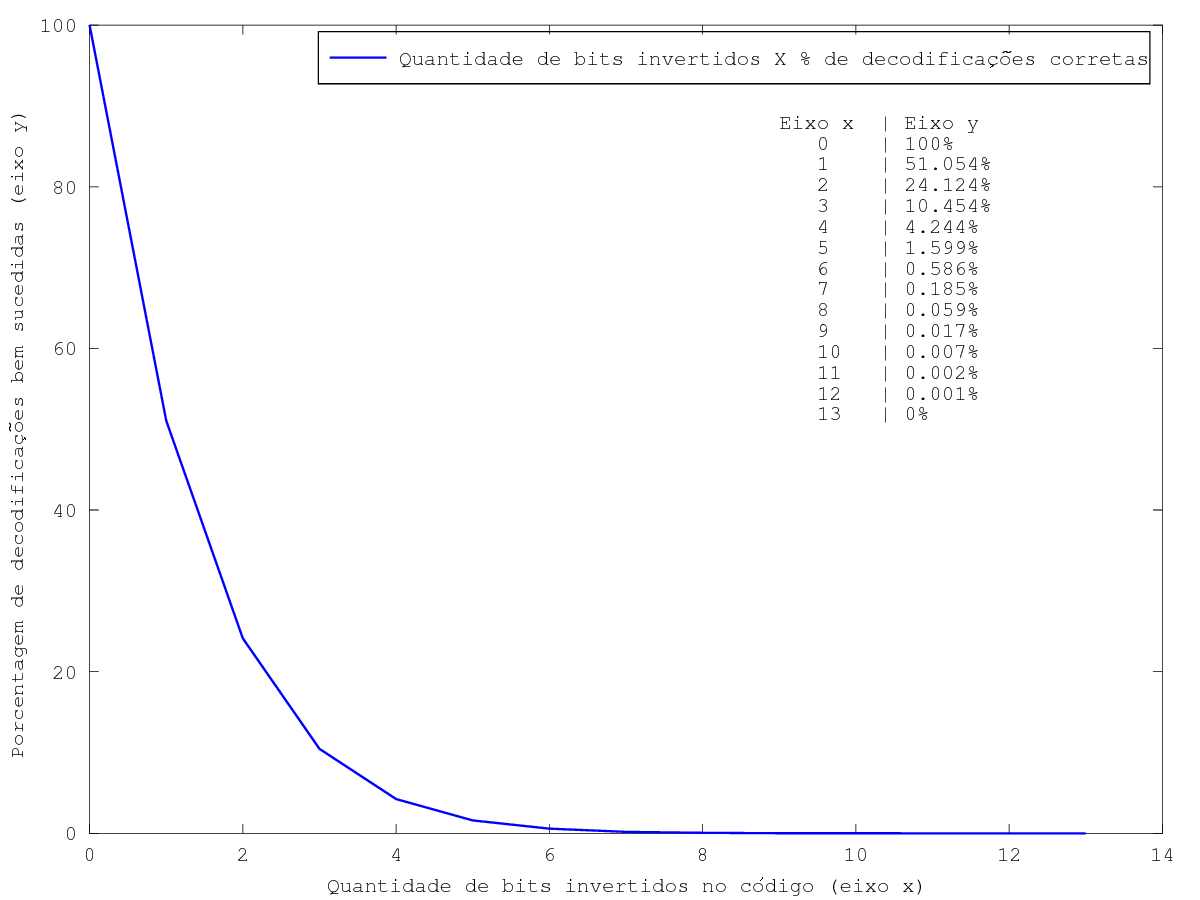
\includegraphics[scale=0.6]{plot.png}
\end{figure}

Através da análise da Figura \ref{fig:cod100} pode-se observar que, para 0\% de ruído, em 100\% dos casos o algoritmo conseguiu recuperar a entrada original, o que de fato já era esperado. Por sua vez, para 1 bit modificado, em 51.054\% dos casos (ou seja, para 51054 execuções dentre as 100000 realizadas) o algoritmo conseguiu recuperar a entrada original. Para 2 bits modificados a decodificação bem sucedida ocorreu em 24.124\% das vezes (em 24124  execuções dentre as 100000 realizadas). Essa taxa decai a medida que a quantidade de bits invertidos no código aumenta, até que para 12 bits modificados têm-se somente uma decodificação bem sucedida entre as 100000 executadas para uma mesma taxa de erro. Para uma quantidade igual ou superior a 13 bits alterados o algoritmo não se mostrou capaz de recuperar a entrada original sem erros.

O mesmo teste também foi aplicado para outras sequências de bits. Como os resultados para elas foram semelhantes às taxas encontradas no exemplo comentado, julgou-se desnecessária sua apresentação. Ainda, cabe destacar que os resultados desse teste mostram a eficiência do codificador/decodificador convolucional, que dentro de faixas de 100000 execuções conseguiu obter resultados de sucesso para casos com até 12 bits alterados. Também é perceptível através desse teste que o algoritmo de fato toma de maneira uniforme caminhos aleatórios de menor erro em casos em que há empate de caminhos com uma mesma taxa mínima de erro, motivo pelo qual em algumas execuções ele conseguiu decodificar com sucesso a sequência de bits e em outras não.

Outro teste realizado foi através da verificação da sequência de resultados de cada uma das etapas do algoritmo. Para isso, foram criadas algumas entradas, executado o algoritmo para essas e impresso no console as sequências de bit de entrada, o resultado da codificação, da adição de ruído, da decodificação e da comparação dos bits da entrada original e da saída da decodificação. Assim, foi possível analisar todo o processo implementado.

Exemplos de entrada podem ser verificados em \emph{1.in}, \emph{2.in} e \emph{3.in}. Para fins de demonstração do teste mencionado será utilizada a entrada de \emph{2.in}, que por ser formada somente por uns facilita a visualização de qual(is) bit(s) não correspondem à entrada original caso o algoritmo não consiga recuperá-la.

Para a entrada contida em \emph{2.in} e uma porcentagem de ruído de 1\% obteve-se em uma das execuções, por exemplo, os dados apresentados na Tabela \ref{teste2.1}.

\def\arraystretch{1.5}
\begin{ThreePartTable}

\begin{longtable}[!ht]{|V {\dimexpr0.40\textwidth-2\tabcolsep\relax}|V{\dimexpr0.59\textwidth-2\tabcolsep\relax}|}
\caption{Execução do algoritmo para a entrada \emph{2.in} e 1\% de ruído}
\label{teste2.1}\\

\hline \multicolumn{1}{|V {\dimexpr0.40\textwidth-2\tabcolsep\relax}|}{\textbf{Descrição do valor}} & \multicolumn{1}{V{\dimexpr0.59\textwidth-2\tabcolsep\relax}|}{\textbf{Valor}} \\[0.5ex]  \hline\hline
\endfirsthead

\multicolumn{2}{l}%
{{\tablename\ \thetable{} -- Execução do algoritmo para a entrada \emph{2.in} e 1\% de ruído}} \\
\multicolumn{2}{r}{{(conclusão)}}\\
\hline \multicolumn{1}{|V {\dimexpr0.40\textwidth-2\tabcolsep\relax}|}{\textbf{Descrição do valor}} & \multicolumn{1}{V{\dimexpr0.59\textwidth-2\tabcolsep\relax}|}{\textbf{Valor}} \\[0.5ex]  \hline\hline
\endhead

\hline \multicolumn{2}{r}{{(continua)}}\\
\endfoot

\hline \hline
\endlastfoot

\textbf{Sequência inicial de bits} & $ \seqsplit{%
11111111111111111111111111111111111111111111111111111111111111111111111111111111111111111111111111}$\\\hline
\textbf{Sequência de bits codificada} & $ \seqsplit{%
11011010101010101010101010101010101010101010101010101010101010101010101010101010101010101010101010101010101010101010101010101010101010101010101010101010101010101010101010101010101010101010101010100111}$\\\hline
\textbf{Sequência codificada com ruído} & $ \seqsplit{%
110110101010101010101010101010\mlq0\mrq01010101010101010101010101010101010101010101010101010101010101010101010101010101010\mlq0\mrq0101010101010101010101010101010101010101010101010101010101010101010101010101010100111}$ \\\hline
\textbf{Sequência decodificada} & $ \seqsplit{%
11111111111111111111111111111111111111111111111111111111111111111111111111111111111111111111111111}$\\\hline
\textbf{Quantidade de bits diferentes entre a entrada original e a saída decodificada} & $0$\\\hline

\end{longtable}
\end{ThreePartTable}

Note que por consistir em uma entrada codificada em 200 bits e ter sido adicionado 1\% de ruído, 2 bits da sequência codificada foram alterados (1\% de 200 = 2). Os bits alterados podem ser verificados entre aspas simples na linha ``Sequência codificada com ruído'' na Tabela \ref{teste2.1}. Ademais, a linha indicando a quantidade de bits diferentes entre a entrada original e a saída decodificada aponta que essa diferença é igual a 0, ou seja, que ambas são iguais (o que significa que o processo de codificação/decodificação foi bem sucedido). Isso também pode ser verificado se compararmos os valores das linhas ``Sequência inicial de bits'' e ``Sequência decodificada'' da Tabela \ref{teste2.1}.

Por sua vez, para a mesma entrada e uma porcentagem de ruído de 2\% obteve-se em uma das execuções, por exemplo, os dados apresentados na Tabela \ref{teste2.2}.

\def\arraystretch{1.5}
\begin{ThreePartTable}

\begin{longtable}[!ht]{|V {\dimexpr0.40\textwidth-2\tabcolsep\relax}|V{\dimexpr0.59\textwidth-2\tabcolsep\relax}|}
\caption{Execução do algoritmo para a entrada \emph{2.in} e 2\% de ruído}
\label{teste2.2}\\

\hline \multicolumn{1}{|V {\dimexpr0.40\textwidth-2\tabcolsep\relax}|}{\textbf{Descrição do valor}} & \multicolumn{1}{V{\dimexpr0.59\textwidth-2\tabcolsep\relax}|}{\textbf{Valor}} \\[0.5ex]  \hline\hline
\endfirsthead

\multicolumn{2}{l}%
{{\tablename\ \thetable{} -- Execução do algoritmo para a entrada \emph{2.in} e 2\% de ruído}} \\
\multicolumn{2}{r}{{(conclusão)}}\\
\hline \multicolumn{1}{|V {\dimexpr0.40\textwidth-2\tabcolsep\relax}|}{\textbf{Descrição do valor}} & \multicolumn{1}{V{\dimexpr0.59\textwidth-2\tabcolsep\relax}|}{\textbf{Valor}} \\[0.5ex]  \hline\hline
\endhead

\hline \multicolumn{2}{r}{{(continua)}}\\
\endfoot

\hline \hline
\endlastfoot

\textbf{Sequência inicial de bits} & $ \seqsplit{%
11111111111111111111111111111111111111111111111111111111111111111111111111111111111111111111111111}$\\\hline
\textbf{Sequência de bits codificada} & $ \seqsplit{%
11011010101010101010101010101010101010101010101010101010101010101010101010101010101010101010101010101010101010101010101010101010101010101010101010101010101010101010101010101010101010101010101010100111}$\\\hline
\textbf{Sequência codificada com ruído} & $ \seqsplit{%
11011\mlq1\mrq10101010101010101010101\mlq1\mrq1010101010101010101010101010101010101010101010101010101\mlq1\mrq1010101010101010101010101010101010101010101010101010101010101010101010101010\mlq0\mrq0101010101010101010101010101010100111}$\\\hline
\textbf{Sequência decodificada} & $ \seqsplit{%
111111111111111111111111111111111111111111\mlq0\mrq1111111111111111111111111111111111111111111111111111111}$\\\hline
\textbf{Quantidade de bits diferentes entre a entrada original e a saída decodificada} & 1\\\hline

\end{longtable}
\end{ThreePartTable}

Esta saída foi tomada a fim de apresentar uma decodificação sem sucesso.

Note que por consistir em uma entrada codificada em 200 bits e ter sido adicionado 2\% de ruído, 4 bits da sequência codificada foram alterados (2\% de 200 = 4). Os bits alterados podem ser verificados entre aspas simples na linha ``Sequência codificada com ruído'' na Tabela \ref{teste2.2}. Ademais, a linha indicando a quantidade de bits diferentes entre a entrada original e a saída decodificada aponta que essa diferença é igual a 1, ou seja, que ambas diferem em um bit. O bit diferente pode ser verificado entre aspas simples na linha ``Sequência decodificada'' da Tabela \ref{teste2.2} ou através de comparação das linhas  ``Sequência inicial de bits'' e ``Sequência decodificada'' da mesma tabela.

Através dos exemplos contidos nas Tabelas \ref{teste2.1} e \ref{teste2.2} puderam ser exemplificados testes de cada uma das etapas do algoritmo para um caso de decodificação bem sucedida e para um caso de decodificação sem sucesso.

Por fim, cabe destacar que a partir dos testes realizados observou-se que o algoritmo implementado atendeu ao propósito ao qual foi desenvolvido, consistindo em um codificador/decodificador convolucional utilizando o Algoritmo de Viterbi, também apresentando bons resultados à tarefa a qual se propõe.

\bibliographystyle{sbc}
\bibliography{sbc-template}

\end{document}